% Options for packages loaded elsewhere
\PassOptionsToPackage{unicode}{hyperref}
\PassOptionsToPackage{hyphens}{url}
%
\documentclass[
  letterpaper,
]{book}

\usepackage{amsmath,amssymb}
\usepackage{iftex}
\ifPDFTeX
  \usepackage[T1]{fontenc}
  \usepackage[utf8]{inputenc}
  \usepackage{textcomp} % provide euro and other symbols
\else % if luatex or xetex
  \usepackage{unicode-math}
  \defaultfontfeatures{Scale=MatchLowercase}
  \defaultfontfeatures[\rmfamily]{Ligatures=TeX,Scale=1}
\fi
\usepackage{lmodern}
\ifPDFTeX\else  
    % xetex/luatex font selection
  \setmainfont[]{Mont}
\fi
% Use upquote if available, for straight quotes in verbatim environments
\IfFileExists{upquote.sty}{\usepackage{upquote}}{}
\IfFileExists{microtype.sty}{% use microtype if available
  \usepackage[]{microtype}
  \UseMicrotypeSet[protrusion]{basicmath} % disable protrusion for tt fonts
}{}
\makeatletter
\@ifundefined{KOMAClassName}{% if non-KOMA class
  \IfFileExists{parskip.sty}{%
    \usepackage{parskip}
  }{% else
    \setlength{\parindent}{0pt}
    \setlength{\parskip}{6pt plus 2pt minus 1pt}}
}{% if KOMA class
  \KOMAoptions{parskip=half}}
\makeatother
\usepackage{xcolor}
\setlength{\emergencystretch}{3em} % prevent overfull lines
\setcounter{secnumdepth}{5}
% Make \paragraph and \subparagraph free-standing
\ifx\paragraph\undefined\else
  \let\oldparagraph\paragraph
  \renewcommand{\paragraph}[1]{\oldparagraph{#1}\mbox{}}
\fi
\ifx\subparagraph\undefined\else
  \let\oldsubparagraph\subparagraph
  \renewcommand{\subparagraph}[1]{\oldsubparagraph{#1}\mbox{}}
\fi


\providecommand{\tightlist}{%
  \setlength{\itemsep}{0pt}\setlength{\parskip}{0pt}}\usepackage{longtable,booktabs,array}
\usepackage{calc} % for calculating minipage widths
% Correct order of tables after \paragraph or \subparagraph
\usepackage{etoolbox}
\makeatletter
\patchcmd\longtable{\par}{\if@noskipsec\mbox{}\fi\par}{}{}
\makeatother
% Allow footnotes in longtable head/foot
\IfFileExists{footnotehyper.sty}{\usepackage{footnotehyper}}{\usepackage{footnote}}
\makesavenoteenv{longtable}
\usepackage{graphicx}
\makeatletter
\def\maxwidth{\ifdim\Gin@nat@width>\linewidth\linewidth\else\Gin@nat@width\fi}
\def\maxheight{\ifdim\Gin@nat@height>\textheight\textheight\else\Gin@nat@height\fi}
\makeatother
% Scale images if necessary, so that they will not overflow the page
% margins by default, and it is still possible to overwrite the defaults
% using explicit options in \includegraphics[width, height, ...]{}
\setkeys{Gin}{width=\maxwidth,height=\maxheight,keepaspectratio}
% Set default figure placement to htbp
\makeatletter
\def\fps@figure{htbp}
\makeatother

\makeatletter
\@ifpackageloaded{tcolorbox}{}{\usepackage[skins,breakable]{tcolorbox}}
\@ifpackageloaded{fontawesome5}{}{\usepackage{fontawesome5}}
\definecolor{quarto-callout-color}{HTML}{909090}
\definecolor{quarto-callout-note-color}{HTML}{0758E5}
\definecolor{quarto-callout-important-color}{HTML}{CC1914}
\definecolor{quarto-callout-warning-color}{HTML}{EB9113}
\definecolor{quarto-callout-tip-color}{HTML}{00A047}
\definecolor{quarto-callout-caution-color}{HTML}{FC5300}
\definecolor{quarto-callout-color-frame}{HTML}{acacac}
\definecolor{quarto-callout-note-color-frame}{HTML}{4582ec}
\definecolor{quarto-callout-important-color-frame}{HTML}{d9534f}
\definecolor{quarto-callout-warning-color-frame}{HTML}{f0ad4e}
\definecolor{quarto-callout-tip-color-frame}{HTML}{02b875}
\definecolor{quarto-callout-caution-color-frame}{HTML}{fd7e14}
\makeatother
\makeatletter
\makeatother
\makeatletter
\@ifpackageloaded{bookmark}{}{\usepackage{bookmark}}
\makeatother
\makeatletter
\@ifpackageloaded{caption}{}{\usepackage{caption}}
\AtBeginDocument{%
\ifdefined\contentsname
  \renewcommand*\contentsname{Содержание}
\else
  \newcommand\contentsname{Содержание}
\fi
\ifdefined\listfigurename
  \renewcommand*\listfigurename{Список Иллюстраций}
\else
  \newcommand\listfigurename{Список Иллюстраций}
\fi
\ifdefined\listtablename
  \renewcommand*\listtablename{Список Таблиц}
\else
  \newcommand\listtablename{Список Таблиц}
\fi
\ifdefined\figurename
  \renewcommand*\figurename{Рисунок}
\else
  \newcommand\figurename{Рисунок}
\fi
\ifdefined\tablename
  \renewcommand*\tablename{Таблица}
\else
  \newcommand\tablename{Таблица}
\fi
}
\@ifpackageloaded{float}{}{\usepackage{float}}
\floatstyle{ruled}
\@ifundefined{c@chapter}{\newfloat{codelisting}{h}{lop}}{\newfloat{codelisting}{h}{lop}[chapter]}
\floatname{codelisting}{Список}
\newcommand*\listoflistings{\listof{codelisting}{Список Каталогов}}
\makeatother
\makeatletter
\@ifpackageloaded{caption}{}{\usepackage{caption}}
\@ifpackageloaded{subcaption}{}{\usepackage{subcaption}}
\makeatother
\makeatletter
\@ifpackageloaded{tcolorbox}{}{\usepackage[skins,breakable]{tcolorbox}}
\makeatother
\makeatletter
\@ifundefined{shadecolor}{\definecolor{shadecolor}{rgb}{.97, .97, .97}}
\makeatother
\makeatletter
\makeatother
\makeatletter
\makeatother
\ifLuaTeX
\usepackage[bidi=basic]{babel}
\else
\usepackage[bidi=default]{babel}
\fi
\babelprovide[main,import]{russian}
% get rid of language-specific shorthands (see #6817):
\let\LanguageShortHands\languageshorthands
\def\languageshorthands#1{}
\ifLuaTeX
  \usepackage{selnolig}  % disable illegal ligatures
\fi
\IfFileExists{bookmark.sty}{\usepackage{bookmark}}{\usepackage{hyperref}}
\IfFileExists{xurl.sty}{\usepackage{xurl}}{} % add URL line breaks if available
\urlstyle{same} % disable monospaced font for URLs
\hypersetup{
  pdftitle={Greek-Slavonic Parallel Corpus},
  pdfauthor={Лев Шадрин, Анастасия Дрожжина},
  pdflang={ru},
  hidelinks,
  pdfcreator={LaTeX via pandoc}}

\title{Greek-Slavonic Parallel Corpus}
\author{Лев Шадрин, Анастасия Дрожжина}
\date{2023-04-07}

\begin{document}
\frontmatter
\maketitle
\ifdefined\Shaded\renewenvironment{Shaded}{\begin{tcolorbox}[interior hidden, boxrule=0pt, frame hidden, borderline west={3pt}{0pt}{shadecolor}, enhanced, sharp corners, breakable]}{\end{tcolorbox}}\fi

\renewcommand*\contentsname{Содержание}
{
\setcounter{tocdepth}{2}
\tableofcontents
}
\mainmatter
\bookmarksetup{startatroot}

\hypertarget{sec-about_project}{%
\chapter{О проекте}\label{sec-about_project}}

Проект \emph{Greek-Slavonic Parallel Corpus} (GSPC) является результатом
работы студентов магистратуры ``Цифровые методы в гуманитарных науках''
НИУ ВШЭ.

Цель проекта -- создание алгоритма выравнивания богослужебных текстов
сложной структуры внутри билингвального корпуса. На данном этапе работы
для проектирования алгоритма используются тексты Цветной Триоди на
греческом и церковнославянском языках.

Работа над проектом началась в декабре 2021 года в рамках
научно-исследовательского проектного семинара программы ``Цифровые
методы в гуманитарных науках'' НИУ-ВШЭ.

\hypertarget{sec-authors}{%
\section{Участники}\label{sec-authors}}

\begin{itemize}
\item
  Шадрин Лев \texttt{leo.shadrin@gmail.com}
\item
  Дрожжина Анастасия \texttt{drozhzhinastya@gmail.com}
\end{itemize}

\hypertarget{sec-acknowledgements}{%
\section{Незаменимые помощники проекта}\label{sec-acknowledgements}}

\begin{itemize}
\item
  \emph{куратор проекта}:\\
  игумен Пантелеимон (Королев), настоятель Данилова монастыря в
  Переславле-Залесском
\item
  \emph{консультационная поддержка}:\\
  Анастасия Александровна Бонч-Осмоловская, кан. филол. наук, доцент
  НИУ-ВШЭ
\end{itemize}

\hfill\break

\bookmarksetup{startatroot}

\hypertarget{sec-about_pent}{%
\chapter{Цветная Триодь}\label{sec-about_pent}}

Цветная Триодь включает в себя богослужебные последования пасхального
цикла, то есть круг подвижных праздников от самой Пасхи до Недели Всех
святых, даты которых меняются в зависимости от дня празднования Пасхи.

Высокая значимость Цветной Триоди как компонента годового круга
церковных служений способствовала выбору этого текста в качестве
материала для нашей работы.

Греческий текст Цветной Триоди выгружен с
\href{https://glt.goarch.org/\#04}{сайта Греческой православной
архиепископии Америки}.

Церковнославянский текст Цветной Триоди выгружен с
\href{https://azbyka.ru/otechnik/Pravoslavnoe_Bogosluzhenie/triod-tsvetnaja/}{сайта
проекта «Азбука веры»}.

\hypertarget{sec-about_pent_specifics}{%
\section{Специфика текста Цветной
Триоди}\label{sec-about_pent_specifics}}

Ниже перечислены особенности текста Цветной Триоди, которые мы выявили и
сформулировали в процессе работы над выравниванием корпуса.

Для каждой особенности предлагается потенциальное направление поиска
решений в контексте дальнейшей работы над проектом.

\hypertarget{sec-temporal_structure}{%
\subsection{Темпоральная структура}\label{sec-temporal_structure}}

Цветная триодь имеет строгую внутреннюю временную структуру, которая
включает в себя следующие уровни:

\begin{itemize}
\item
  Неделя

  \begin{itemize}
  \item
    День недели

    \begin{itemize}
    \tightlist
    \item
      Служба
    \end{itemize}
  \end{itemize}
\end{itemize}

\begin{quote}
Говоря об этой книге, как и о любой другой, мы должны прежде всего знать
границы ее действия. Триодь Цветная употребляется с утрени первого дня
Пасхи до Божественной литургии в Неделю Всех святых, когда в последний
раз поются песнопения Триоди Цветной, а в заключение написано: «Конец и
Богу слава». Такой огромный период, конечно, распадается на составные
части. Безусловно, выделяется первый день Пасхи и Пасхальная седмица;
затем имеет общие законы богослужения время от Фоминой недели до отдания
Пасхи; Вознесение с попразднством, Троица (Пятидесятница) с
попразднством и последний день пения Триоди Цветной -- Неделя Всех
святых.\footnote{М.С. Красовицкая, ``Литургика''. Лекция 19.
  Богослужение в период пения триоди цветной. Доступно по
  \href{https://azbyka.ru/otechnik/Pravoslavnoe_Bogosluzhenie/liturgika-krasovitskaja/19}{ссылке}}
\end{quote}

\begin{tcolorbox}[enhanced jigsaw, breakable, arc=.35mm, colframe=quarto-callout-note-color-frame, leftrule=.75mm, bottomrule=.15mm, rightrule=.15mm, toprule=.15mm, opacityback=0, left=2mm, colback=white]

\textbf{Что это значит в контексте задачи?}\vspace{2mm}

На уровне темпоральной организации от элайнера ожидается строгое
выравнивание элементов в билингвальном корпусе: неделя к неделе, день ко
дню, служба к службе. Если подобное выравнивание не достигается
автоматически\footnotemark{}, требуется предварительная разметка текста,
которая позволила бы провести частичное выравнивание на более низких
уровнях, с поэтапным масштабированием

\end{tcolorbox}

\footnotetext{Подробнее о результатах работы элайнеров см. раздел о
\protect\hyperlink{sec-about_aligners}{готовых решениях}, а также раздел
\protect\hyperlink{sec-about_evluation}{об оценке качества}}

\hypertarget{sec-func_structure}{%
\subsection{Функциональная структура}\label{sec-func_structure}}

Внутри текста Цветной Триоди можно выделить 2 уровня:

\begin{itemize}
\item
  служебные комментариями по организации и проведению службы
\item
  тексты молитв и песнопений
\end{itemize}

В рукописной традиции элементы различных уровней текста выделяются
особым образом -- от размера буквиц и инициалов до использования
маюскульных шрифтов или вязи в заглавиях. Любопытно, что данная традиция
находит и современное цифровое воплощение: на сайтах, которые
использовались в качестве источников текстов для настоящего проекта,
элементы разных уровней маркированы при помощи цвета.

Так, тексты молитв отображаются привычным черным цветом, а служебные
указания выделены ``киноварью'' - красным.

\begin{tcolorbox}[enhanced jigsaw, breakable, arc=.35mm, colframe=quarto-callout-tip-color-frame, leftrule=.75mm, bottomrule=.15mm, rightrule=.15mm, toprule=.15mm, opacityback=0, left=2mm, colback=white]

\textbf{Как это выглядит на сайте ``Азбуки''?}\vspace{2mm}

\begin{figure}[H]

{\centering 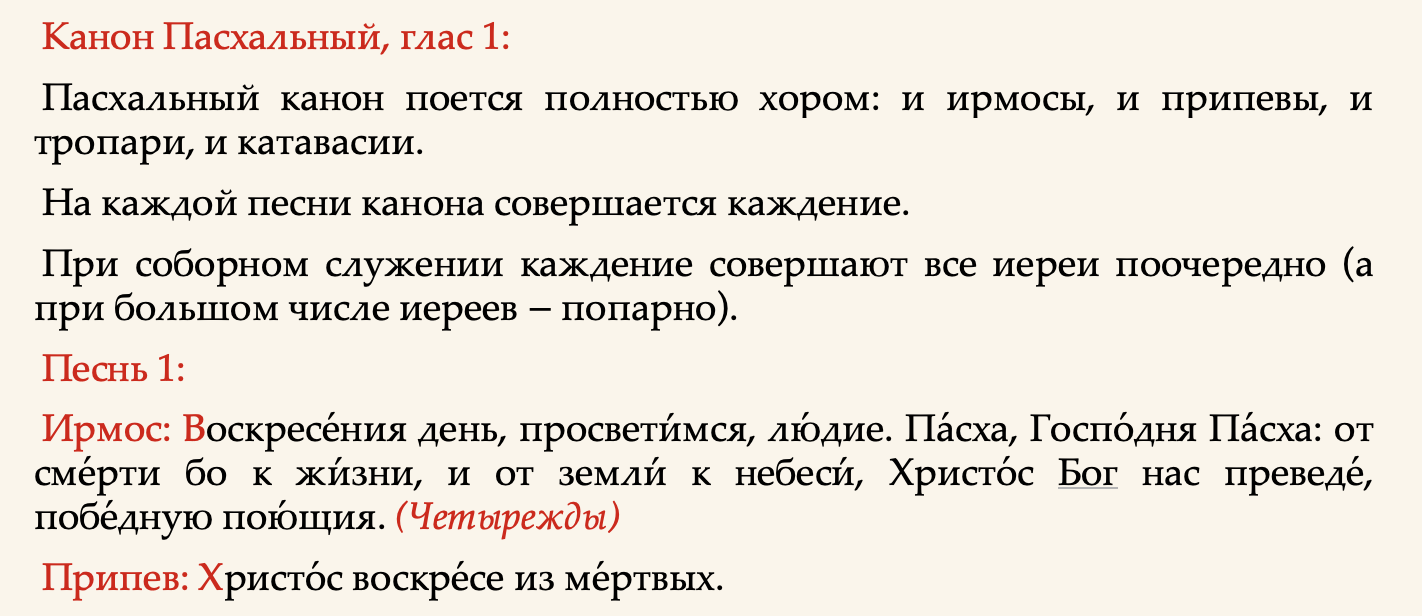
\includegraphics[width=0.75\textwidth,height=\textheight]{images/pascha_canon_csl.png}

}

\end{figure}

Киноварью выделены заголовки и указание \emph{``Четырежды''}

\end{tcolorbox}

Подробнее о работе с цветовой разметкой см. в разделе о
\protect\hyperlink{sec-html_color}{предобработке текстов}.

\begin{tcolorbox}[enhanced jigsaw, breakable, arc=.35mm, colframe=quarto-callout-note-color-frame, leftrule=.75mm, bottomrule=.15mm, rightrule=.15mm, toprule=.15mm, opacityback=0, left=2mm, colback=white]

\textbf{Почему так важен цвет ``цифрового'' текста?}\vspace{2mm}

Бинарная функциональная структура является одной из причин расхождения
длины богослужебных текстов для разных языков. Так, в греческом тексте
Цветной Триоди служебные комментарии представлены в значительно
сокращенном виде по сравнению со схожими элементами церковнославянского
текста

\end{tcolorbox}

\hypertarget{sec-element_order}{%
\subsection{Порядок следования фрагментов}\label{sec-element_order}}

Тексты песнопений на различных языках могут иметь отличный друг от друга
порядок следований, что создает перекрестную структуру внутри
билингвального корпуса и значительно усложняет задачу параллельного
выравнивания.

\begin{tcolorbox}[enhanced jigsaw, breakable, arc=.35mm, colframe=quarto-callout-note-color-frame, leftrule=.75mm, bottomrule=.15mm, rightrule=.15mm, toprule=.15mm, opacityback=0, left=2mm, colback=white]

\textbf{Почему это важно для нас?}\vspace{2mm}

Разрозненный порядок следования молитв внутри элементов службы или дня
затрудняет работу классических элайнеров (см. раздел
\protect\hyperlink{sec-about_aligners}{Готовые решения}). Необходимо
устанавливать широкое окно для оценки близости различных компонентов

\end{tcolorbox}

\hypertarget{sec-full_or_abridged_hymns}{%
\subsection{Тексты молитв: краткие и полные
варианты}\label{sec-full_or_abridged_hymns}}

В текстах Цветной Триоди на обоих языках молитвы могут быть представлены
как в сокращенном формате, так и целиком.

После текста молитвы может следовать краткое служебное указание о
повторении молитвы. В иных случаях, текст молитвы может дублироваться
полностью в последующих абзацах, повторяясь необходимое количество раз
для исполнения во время службы.

\begin{tcolorbox}[enhanced jigsaw, breakable, arc=.35mm, colframe=quarto-callout-tip-color-frame, leftrule=.75mm, bottomrule=.15mm, rightrule=.15mm, toprule=.15mm, opacityback=0, left=2mm, colback=white]

\textbf{Пример: Пасхальный канон}\vspace{2mm}

Так, приведенному выше фрагменту Пасхального канона в церковнославянском
тексте предшествует подробное указание:

\begin{quote}
И начина́ет предстоя́тель кано́н, творе́ние Господи́на иоа́нна дамаскина́. Гла́с
1. Ирмо́с:~Воскресе́ния де́нь: Ирмосы́ на 4:~И тропари́ на 12, с
припе́вы:~Христо́с воскре́се из ме́ртвых.~И па́ки последи́ ки́йждо ли́к ирмо́с.
Последи́ же на схо́де катава́сиа, ирмо́с то́йже:~Воскресе́ния де́нь:~И по не́м:
Христо́с воскре́се: ве́сь три́жды.Твори́т же нача́ло кано́на на ку́юждо пе́снь
всегда́ предстоя́тель, десно́й или́ ле́вой стране́ случи́вшейся нача́ти. И кади́т
в нача́ле кано́на святы́я ико́ны, и о́ба ли́ки и бра́тию по чи́ну. И по ко́ейждо
пе́сни быва́ет ектениа́ ма́лая вне́ олтаря́, я́коже ре́хом, во святы́й се́й де́нь.
Возгла́с вну́трь олтаря́ от иере́а. По 1-й пе́сни пое́т десна́я страна́. По 3-й
же пое́т ле́вая. Си́це пое́м и по про́чих пе́снех.

Канон Пасхальный, глас 1:

Пасхальный канон поется полностью хором: и ирмосы, и припевы, и тропари,
и катавасии.

На каждой песни канона совершается каждение.

При соборном служении каждение совершают все иереи поочередно (а при
большом числе иереев -- попарно).

Песнь 1:

Ирмос: Воскресе́ния день, просвети́мся, лю́дие.
\textless\ldots\textgreater{}
\end{quote}

Этот же фрагмент службы в греческом языке не содержит эквивалентных
указаний:

\begin{quote}
Ὁ Κανών, ποίημα Ἰωάννου τοῦ Δαμασκηνοῦ.

ᾨδὴ α' Ἦχος α' εἱρμὸς

«Ἀναστάσεως ἡμέρα λαμπρυνθῶμεν Λαοί \textless\ldots\textgreater{}
\end{quote}

\end{tcolorbox}

\begin{tcolorbox}[enhanced jigsaw, breakable, arc=.35mm, colframe=quarto-callout-note-color-frame, leftrule=.75mm, bottomrule=.15mm, rightrule=.15mm, toprule=.15mm, opacityback=0, left=2mm, colback=white]

\textbf{Что можно с этим сделать?}\vspace{2mm}

Для решения задачи по выравниванию корпуса требуется нормализация
подобных сводимых элементов.

\end{tcolorbox}

\bookmarksetup{startatroot}

\hypertarget{ux43fux440ux438ux43cux435ux440-ux43fux430ux441ux445ux430ux43bux44cux43dux44bux439-ux43aux430ux43dux43eux43d-ux438ux43eux430ux43dux43dux430-ux434ux430ux43cux430ux441ux43aux438ux43dux430}{%
\chapter{Пример: Пасхальный канон Иоанна
Дамаскина}\label{ux43fux440ux438ux43cux435ux440-ux43fux430ux441ux445ux430ux43bux44cux43dux44bux439-ux43aux430ux43dux43eux43d-ux438ux43eux430ux43dux43dux430-ux434ux430ux43cux430ux441ux43aux438ux43dux430}}

Посмотрим еще раз на фрагмент Пасхального канона Иоанна Дамаскина. Ниже
приведены части текстов в том порядке, в каком они представлены в
источниках.

\begin{tcolorbox}[enhanced jigsaw, breakable, arc=.35mm, colframe=quarto-callout-tip-color-frame, leftrule=.75mm, bottomrule=.15mm, rightrule=.15mm, toprule=.15mm, opacityback=0, left=2mm, colback=white]

\textbf{Фрагмент церковнославянского текста}\vspace{2mm}

Канон Пасхальный, глас 1:

Пасхальный канон поется полностью хором: и ирмосы, и припевы, и тропари,
и катавасии.

На каждой песни канона совершается каждение.

При соборном служении каждение совершают все иереи поочередно (а при
большом числе иереев -- попарно).

Песнь 1:

Ирмос: Воскресе́ния день, просвети́мся, лю́дие. Па́сха, Госпо́дня Па́сха: от
сме́рти бо к жи́зни, и от земли́ к небеси́, Христо́с~Бог~нас преведе́,
побе́дную пою́щия.~(Четырежды)

Припев: Христо́с воскре́се из ме́ртвых.

Очи́стим чу́вствия, и у́зрим непристу́пным све́том Воскресе́ния, Христа́
блиста́ющася, и ра́дуйтеся, реку́ща, я́сно да услы́шим, побе́дную пою́ще. (6
раз)

Небеса́ у́бо досто́йно да веселя́тся, земля́ же да ра́дуется, да пра́зднует же
мир, ви́димый же весь и неви́димый: Христо́с бо воста́, весе́лие ве́чное. (6
раз)

\end{tcolorbox}

\begin{tcolorbox}[enhanced jigsaw, breakable, arc=.35mm, colframe=quarto-callout-tip-color-frame, leftrule=.75mm, bottomrule=.15mm, rightrule=.15mm, toprule=.15mm, opacityback=0, left=2mm, colback=white]

\textbf{Фрагмент греческого текста}\vspace{2mm}

Ὁ Κανών, ποίημα Ἰωάννου τοῦ Δαμασκηνοῦ.

ᾨδὴ α' Ἦχος α' εἱρμὸς

«Ἀναστάσεως ἡμέρα λαμπρυνθῶμεν Λαοί, Πάσχα Κυρίου, Πάσχα· ἐκ γὰρ θανάτου
πρὸς ζωήν, καὶ ἐκ γῆς πρὸς οὐρανόν, Χριστὸς ὁ Θεός, ἡμᾶς διεβίβασεν,
ἐπινίκιον ᾄδοντας».

Καθαρθῶμεν τὰς αἰσθήσεις, καὶ ὀψόμεθα, τῷ ἀπροσίτῳ φωτὶ τῆς ἀναστάσεως,
Χριστὸν ἐξαστράπτοντα, καί, Χαίρετε, φάσκοντα, τρανῶς ἀκουσόμεθα,
ἐπινίκιον ᾄδοντες.

Οὐρανοὶ μὲν ἐπαξίως εὐφραινέσθωσαν, γῆ δὲ ἀγαλλιάσθω, ἑορταζέτω δὲ
κόσμος, ὁρατός τε ἅπας καὶ ἀόρατος· Χριστὸς γὰρ ἐγήγερται, εὐφροσύνη
αἰώνιος.

\end{tcolorbox}

Если постараться выделить индивидуальные элементы и свести их вручную,
стараясь сохранить последовательность, то получится следующая структура:

\begin{longtable}[]{@{}
  >{\raggedright\arraybackslash}p{(\columnwidth - 2\tabcolsep) * \real{0.5900}}
  >{\raggedright\arraybackslash}p{(\columnwidth - 2\tabcolsep) * \real{0.4100}}@{}}
\toprule\noalign{}
\endhead
\bottomrule\noalign{}
\endlastfoot
\textbf{Церковнославянский} & \textbf{Греческий} \\
Канон Пасхальный, & Ὁ Κανών, \\
глас 1: & - \\
- & ποίημα Ἰωάννου τοῦ Δαμασκηνοῦ. \\
Пасхальный канон поется полностью хором: и ирмосы, и припевы, и тропари,
и катавасии. На каждой песни канона совершается каждение. При соборном
служении каждение совершают все иереи поочередно (а при большом числе
иереев -- попарно). & - \\
Песнь 1: & ᾨδὴ α' \\
- & Ἦχος α' \\
Ирмос: & εἱρμὸς \\
Воскресе́ния день, просвети́мся, лю́дие. Па́сха, Госпо́дня Па́сха: от сме́рти
бо к жи́зни, и от земли́ к небеси́, Христо́с~Бог~нас преведе́, побе́дную
пою́щия. & «Ἀναστάσεως ἡμέρα λαμπρυνθῶμεν Λαοί, Πάσχα Κυρίου, Πάσχα· ἐκ
γὰρ θανάτου πρὸς ζωήν, καὶ ἐκ γῆς πρὸς οὐρανόν, Χριστὸς ὁ Θεός, ἡμᾶς
διεβίβασεν, ἐπινίκιον ᾄδοντας». \\
Припев: Христо́с воскре́се из ме́ртвых. & - \\
Очи́стим чу́вствия, и у́зрим непристу́пным све́том Воскресе́ния, Христа́
блиста́ющася, и ра́дуйтеся, реку́ща, я́сно да услы́шим, побе́дную пою́ще. &
Καθαρθῶμεν τὰς αἰσθήσεις, καὶ ὀψόμεθα, τῷ ἀπροσίτῳ φωτὶ τῆς ἀναστάσεως,
Χριστὸν ἐξαστράπτοντα, καί, Χαίρετε, φάσκοντα, τρανῶς ἀκουσόμεθα,
ἐπινίκιον ᾄδοντες. \\
(6 раз) & - \\
Небеса́ у́бо досто́йно да веселя́тся, земля́ же да ра́дуется, да пра́зднует же
мир, ви́димый же весь и неви́димый: Христо́с бо воста́, весе́лие ве́чное. &
Οὐρανοὶ μὲν ἐπαξίως εὐφραινέσθωσαν, γῆ δὲ ἀγαλλιάσθω, ἑορταζέτω δὲ
κόσμος, ὁρατός τε ἅπας καὶ ἀόρατος· Χριστὸς γὰρ ἐγήγερται, εὐφροσύνη
αἰώνιος. \\
(6 раз) & - \\
\end{longtable}

На этом примере мы видим комбинацию всех рассмотренных
\protect\hyperlink{sec-about_pent_specifics}{особенностей текста}:

\begin{itemize}
\item
  \textbf{краткие и полные варианты}:

  \begin{itemize}
  \tightlist
  \item
    служебные указания в церковнославянском тексте не имеют эквивалентов
    в греческом
  \end{itemize}
\item
  \textbf{перекрестная структура}:

  \begin{itemize}
  \tightlist
  \item
    элементы \texttt{Глас\ 1} и
    \texttt{Ἦχος\ α\textquotesingle{}}являются эквивалентами, но
    находятся в разных местах в текстах
  \end{itemize}
\item
  \textbf{цветовая структура}:

  \begin{itemize}
  \tightlist
  \item
    киноварные указания могут быть использованы как ``якоря'' для
    улучшения результатов элайнмента
  \end{itemize}
\end{itemize}

\bookmarksetup{startatroot}

\hypertarget{sec-about_preprocessing}{%
\chapter{Предварительная обработка
текстов}\label{sec-about_preprocessing}}

За весь период работы над проектом мы провели большое количество
разнообразных экспериментов по обработке изначальных текстовых данных,
варьируя объем текстов, сочетание структурных единиц, а также методы и
инструменты обработки.

На данный момент мы выявили следующие этапы предобработки текстов,
которые позволяют извлечь и структурировать необходимую для выравнивания
информацию.

\hypertarget{sec-html_color}{%
\section{Выгрузка html и цветовая разметка}\label{sec-html_color}}

На \protect\hyperlink{sec-about_pent}{веб-страницах}, с которых были
выгружены тексты для работы, фрагменты молитв и служебных указаний
размечены при помощи параметров цвета внутри html-тегов.

Тексты молитв выделены черным цветом, указаний - красным. Предположив,
что сохранение данной структуры (см. особенность 2 раздела ``Специфика
текста Цветной триоди (в частности) и богослужебных текстов'') поможет
улучшить результаты выравнивания корпуса, мы решили выгрузить тексты с
сохранением цветовой разметки.

\begin{itemize}
\item
  \textbf{Церковнославянский текст} имел регулярную html-структуру, и
  сведения о цветовой маркировке удалось получить с помощью базовых
  инструментов для веб-скрейпинга и
  \href{https://github.com/Drozhzhinastya/GSPC/blob/main/scripts/scraping/md_to_csv_csl.ipynb}{регулярных
  выражений}
\item
  При работе с html-структурой \textbf{греческого текста} мы столкнулись
  с ошибками в организации страницы: многие текстовые фрагменты не
  попадали в теги цветовой разметки. Для корректной выгрузки греческого
  текста был написан
  \href{https://github.com/Drozhzhinastya/GSPC/blob/main/scripts/scraping/scrape_grc.ipynb}{код}
\end{itemize}

Цветовая маркировка отображается в
\href{https://github.com/Drozhzhinastya/GSPC/tree/main/csv/markup}{csv}
-- текст поделен между колонками \texttt{black\_text} (тексты служб) и
\texttt{red\_text} (комментарии к текстам), сведения о структуре
отражены в столбце \texttt{color} (значения \texttt{red} и
\texttt{black} соответственно).

\begin{tcolorbox}[enhanced jigsaw, breakable, arc=.35mm, colframe=quarto-callout-note-color-frame, leftrule=.75mm, bottomrule=.15mm, rightrule=.15mm, toprule=.15mm, opacityback=0, left=2mm, colback=white]

\textbf{Как это выглядит?}\vspace{2mm}

В таблице ниже приведен пример, иллюстрирующий структуру данных с
информацией о цветовой маркировке текста

\end{tcolorbox}

\begin{longtable}[]{@{}
  >{\raggedright\arraybackslash}p{(\columnwidth - 4\tabcolsep) * \real{0.1667}}
  >{\raggedright\arraybackslash}p{(\columnwidth - 4\tabcolsep) * \real{0.6667}}
  >{\raggedright\arraybackslash}p{(\columnwidth - 4\tabcolsep) * \real{0.1667}}@{}}
\toprule\noalign{}
\begin{minipage}[b]{\linewidth}\raggedright
red\_text
\end{minipage} & \begin{minipage}[b]{\linewidth}\raggedright
black\_text
\end{minipage} & \begin{minipage}[b]{\linewidth}\raggedright
color
\end{minipage} \\
\midrule\noalign{}
\endhead
\bottomrule\noalign{}
\endlastfoot
& Воскре́сение Твое́ Христе́ Спа́се, А́нгели пою́т на небесе́х, и на́с на земли́
сподо́би чи́стым се́рдцем Тебе́ сла́вити. & black \\
И велегла́сно возгласи́т: & & red \\
И на́м отвеща́ющым: & & red \\
\end{longtable}

\hypertarget{sec_temporal_markup}{%
\section{Темпоральная разметка}\label{sec_temporal_markup}}

Темпоральная разметка выполнена вручную, отдельно для греческого и
церковнославянского текстов. Размечены два уровня временной структуры:
недели (\texttt{1} - \texttt{8}) и дни (\texttt{1\_1} - \texttt{8\_8}).

Темпоральная разметка содержится в
\href{https://github.com/Drozhzhinastya/GSPC/tree/main/csv/markup}{csv}
в столбце \texttt{temp}

\begin{tcolorbox}[enhanced jigsaw, breakable, arc=.35mm, colframe=quarto-callout-note-color-frame, leftrule=.75mm, bottomrule=.15mm, rightrule=.15mm, toprule=.15mm, opacityback=0, left=2mm, colback=white]

\textbf{Как это выглядит?}\vspace{2mm}

Ниже показан пример структуры данных с информацией о темпоральной
разметке

\end{tcolorbox}

\begin{longtable}[]{@{}
  >{\raggedright\arraybackslash}p{(\columnwidth - 6\tabcolsep) * \real{0.0945}}
  >{\raggedright\arraybackslash}p{(\columnwidth - 6\tabcolsep) * \real{0.8731}}
  >{\raggedright\arraybackslash}p{(\columnwidth - 6\tabcolsep) * \real{0.0174}}
  >{\raggedright\arraybackslash}p{(\columnwidth - 6\tabcolsep) * \real{0.0149}}@{}}
\toprule\noalign{}
\begin{minipage}[b]{\linewidth}\raggedright
red\_text
\end{minipage} & \begin{minipage}[b]{\linewidth}\raggedright
black\_text
\end{minipage} & \begin{minipage}[b]{\linewidth}\raggedright
color
\end{minipage} & \begin{minipage}[b]{\linewidth}\raggedright
temp
\end{minipage} \\
\midrule\noalign{}
\endhead
\bottomrule\noalign{}
\endlastfoot
ΤΗΣ ΔΙΑΚΑΙΝΗΣΙΜΟΥ & & red & 1 \\
Τῌ ΑΓΙᾼ ΚΑΙ ΜΕΓΑΛῌ ΚΥΡΙΑΚῌ ΤΟΥ ΠΑΣΧΑ & & red & 1\_1 \\
ΕΩΘΙΝΟΝ Ζ' Ἦχος βαρὺς & & red & \\
& Ἰδοὺ σκοτία καὶ πρωΐ, καὶ τί πρὸς τὸ μνημεῖον Μαρία ἕστηκας, πολὺ
σκότος ἔχουσα ταῑς φρεσίν; ὑφ' οὗ ποῦ τέθειται ζητεῖς ὁ Ἰησοῦς. Ἀλλ' ὅρα
τοὺς συντρέχοντας Μαθητάς, πῶς τοῖς ὀθονίοις καὶ τῷ σουδαρίῳ, τὴν
Ἀνάστασιν ἐτεκμήραντο, καὶ ἀνεμνήσθησαν τῆς περὶ τούτου Γραφῆς. Μεθ' ὧν,
καὶ δι' ὧν καὶ ἡμεῖς, πιστεύσαντες, ἀνυμνοῦμέν σε τὸν ζωοδότην Χριστόν.
& black & \\
\end{longtable}

\hypertarget{sec_hymn_sequence}{%
\section{Различный порядок следования молитв и
песнопений}\label{sec_hymn_sequence}}

Оптимальными решениями для работы с этой особенностью служебных текстов,
на наш взгляд являются инструменты, которые позволяют сопоставлять
единицы, находящиеся на большом расстоянии друг от друга в тексте (см.
раздел \protect\hyperlink{text-similarity}{text-similarity})

\hypertarget{ux440ux430ux437ux43bux438ux447ux43dux43eux435-ux43eux444ux43eux440ux43cux43bux435ux43dux438ux435-ux442ux435ux43aux441ux442ux43eux432-ux43cux43eux43bux438ux442ux432}{%
\section{Различное оформление текстов
молитв}\label{ux440ux430ux437ux43bux438ux447ux43dux43eux435-ux43eux444ux43eux440ux43cux43bux435ux43dux438ux435-ux442ux435ux43aux441ux442ux43eux432-ux43cux43eux43bux438ux442ux432}}

Развернутая структура оформления текста молитв сохраняется в csv файлах.
Однако мы предполагаем, что для оптимизации параметров длины исходных
текстов, релевантна работа с
\href{https://github.com/Drozhzhinastya/GSPC/tree/main/texts/unique_units}{уникальными
единицами текста}.

\bookmarksetup{startatroot}

\hypertarget{sec-about_aligners}{%
\chapter{Готовые пакеты решений (элайнеры)}\label{sec-about_aligners}}

На начальных этапах работы мы предполагали использовать элайнеры --
готовые программные решения для задач по выравниванию параллельных
текстов. Мы проводили эксперименты в \textbf{Lingtrain Aligner}, а также
\textbf{Hunalign} и его пользовательскую оболочку LF-aligner. Рассмотрим
каждый из инструментов в отдельности.

\hypertarget{sec-lf_aligner}{%
\section{LF-aligner}\label{sec-lf_aligner}}

\emph{LF-aligner} является графическим интерфейсом для непосредственного
элайнера
\emph{\href{https://github.com/danielvarga/hunalign}{Hunalign}}. Этот
инструмент требует предварительной лемматизации обрабатываемых текстов.
Подробнее о лемматизации можно почитать в
\protect\hyperlink{ux43bux435ux43cux43cux430ux442ux438ux437ux430ux446ux438ux44f}{соответсвующем
разделе}.

Алгоритм \emph{Hunalign} решает задачу выравнивания лемматизированных
текстов по предложениям или параграфам -- что соответствует элементам
молитв в нашем случае.

При работе с \emph{Hunalign} возникает проблема, связанная с отсутствием
возможности настройки параметров окна сравнения единиц текста, из-за
чего инструмент показывает крайне низкое качество сведения при работе со
сложной \protect\hyperlink{sec-element_order}{перекрестной структурой
Цветной Триоди}.

\begin{tcolorbox}[enhanced jigsaw, breakable, arc=.35mm, colframe=quarto-callout-note-color-frame, leftrule=.75mm, bottomrule=.15mm, rightrule=.15mm, toprule=.15mm, opacityback=0, left=2mm, colback=white]

\textbf{Что еще умеет Hunalign?}\vspace{2mm}

В \emph{Hunalign} можно дополнительно подгрузить внешний словарь
переводных эквивалентов -- в таком случае, алгоритм будет использовать
его, комбинируя словарные данные с информацией о длине предложения по
алгоритму Гейла-Черча.\footnotemark{}

В отсутствии внешнего словаря алгоритм сперва обращается к длине
предложения, а затем автоматически генерирует словарь на основе
результатов первичного выравнивания по длине. После этого
\emph{Hunalign} выравнивает текст повторно, используя сгенерированные
словарные данные.

\end{tcolorbox}

\footnotetext{В основе алгоритма лежит принцип, согласно которому
эквивалентные предложения должны примерно соответствовать по длине:
более длинные предложения на одном языке - более длинным предложениям на
другом языке. Подробнее см. в статье Gale W., Church K. A program for
aligning sentences in bilingual corpora
(\href{https:/\%20/web.archive.org/web/20061026051708/http://acl.ldc.upenn.edu/J/J93/J93-1004.pdf}{ссылка
на статью}).}

\hypertarget{sec-lingtrain}{%
\section{Lingtrain-aligner}\label{sec-lingtrain}}

Среди преимуществ работы с
\href{https://github.com/averkij/lingtrain-aligner}{Lingtrain Aligner}
стоит отметить нетребовательность инструмента к предварительной
подготовке текстов, а также относительную простоту запуска алгоритмов
выравнивания.

Пользователю не требуется осуществлять токенизацию и лемматизацию
текста. Необходимо лишь определенным образом
\href{https://habr.com/ru/articles/590549/}{разметить текст} и
убедиться, что он соответствует следующим параметрам:

\begin{itemize}
\tightlist
\item
  в случае если проставлены метки для заголовков, их число должно быть
  одинаковым для обоих текстов;
\item
  в тексте отсутствуют строки, заканчивающиеся точкой и не являющиеся
  концом абзаца; в противном случае, абзацы будут сегментированы по
  точкам
\end{itemize}

Работать с подготовленными корпусами можно из python при помощи
библиотеки lingtrain-aligner.

\hypertarget{html-ux43aux43dux438ux433ux430}{%
\subsection{html-книга}\label{html-ux43aux43dux438ux433ux430}}

Предварительная разметка текста оказывается полезной не только для
выравнивания в элайнерах, но также помогает при создании визуализации
результатов -- \textbf{html-книги} с параллельными текстами.

Формат выдачи результатов в виде html-книги, предусмотренный в
lingtrain, не является оптимальным для целей проекта на данном этапе,
поскольку мы заинтересованы в получении словаря переводных эквивалентов
на уровне отдельных гимнов или предложений, а также в оценке качества
выравнивания.

\begin{tcolorbox}[enhanced jigsaw, breakable, arc=.35mm, colframe=quarto-callout-caution-color-frame, leftrule=.75mm, bottomrule=.15mm, rightrule=.15mm, toprule=.15mm, opacityback=0, left=2mm, colback=white]

\textbf{Посмотреть на результат работы Lingtrain}\vspace{2mm}

Из 8 пар элементов верно свелась лишь одна: \emph{Τὸ Πνεῦμα τὸ
ἄγιον\ldots{}} - \emph{Дух же Святый\ldots{}}

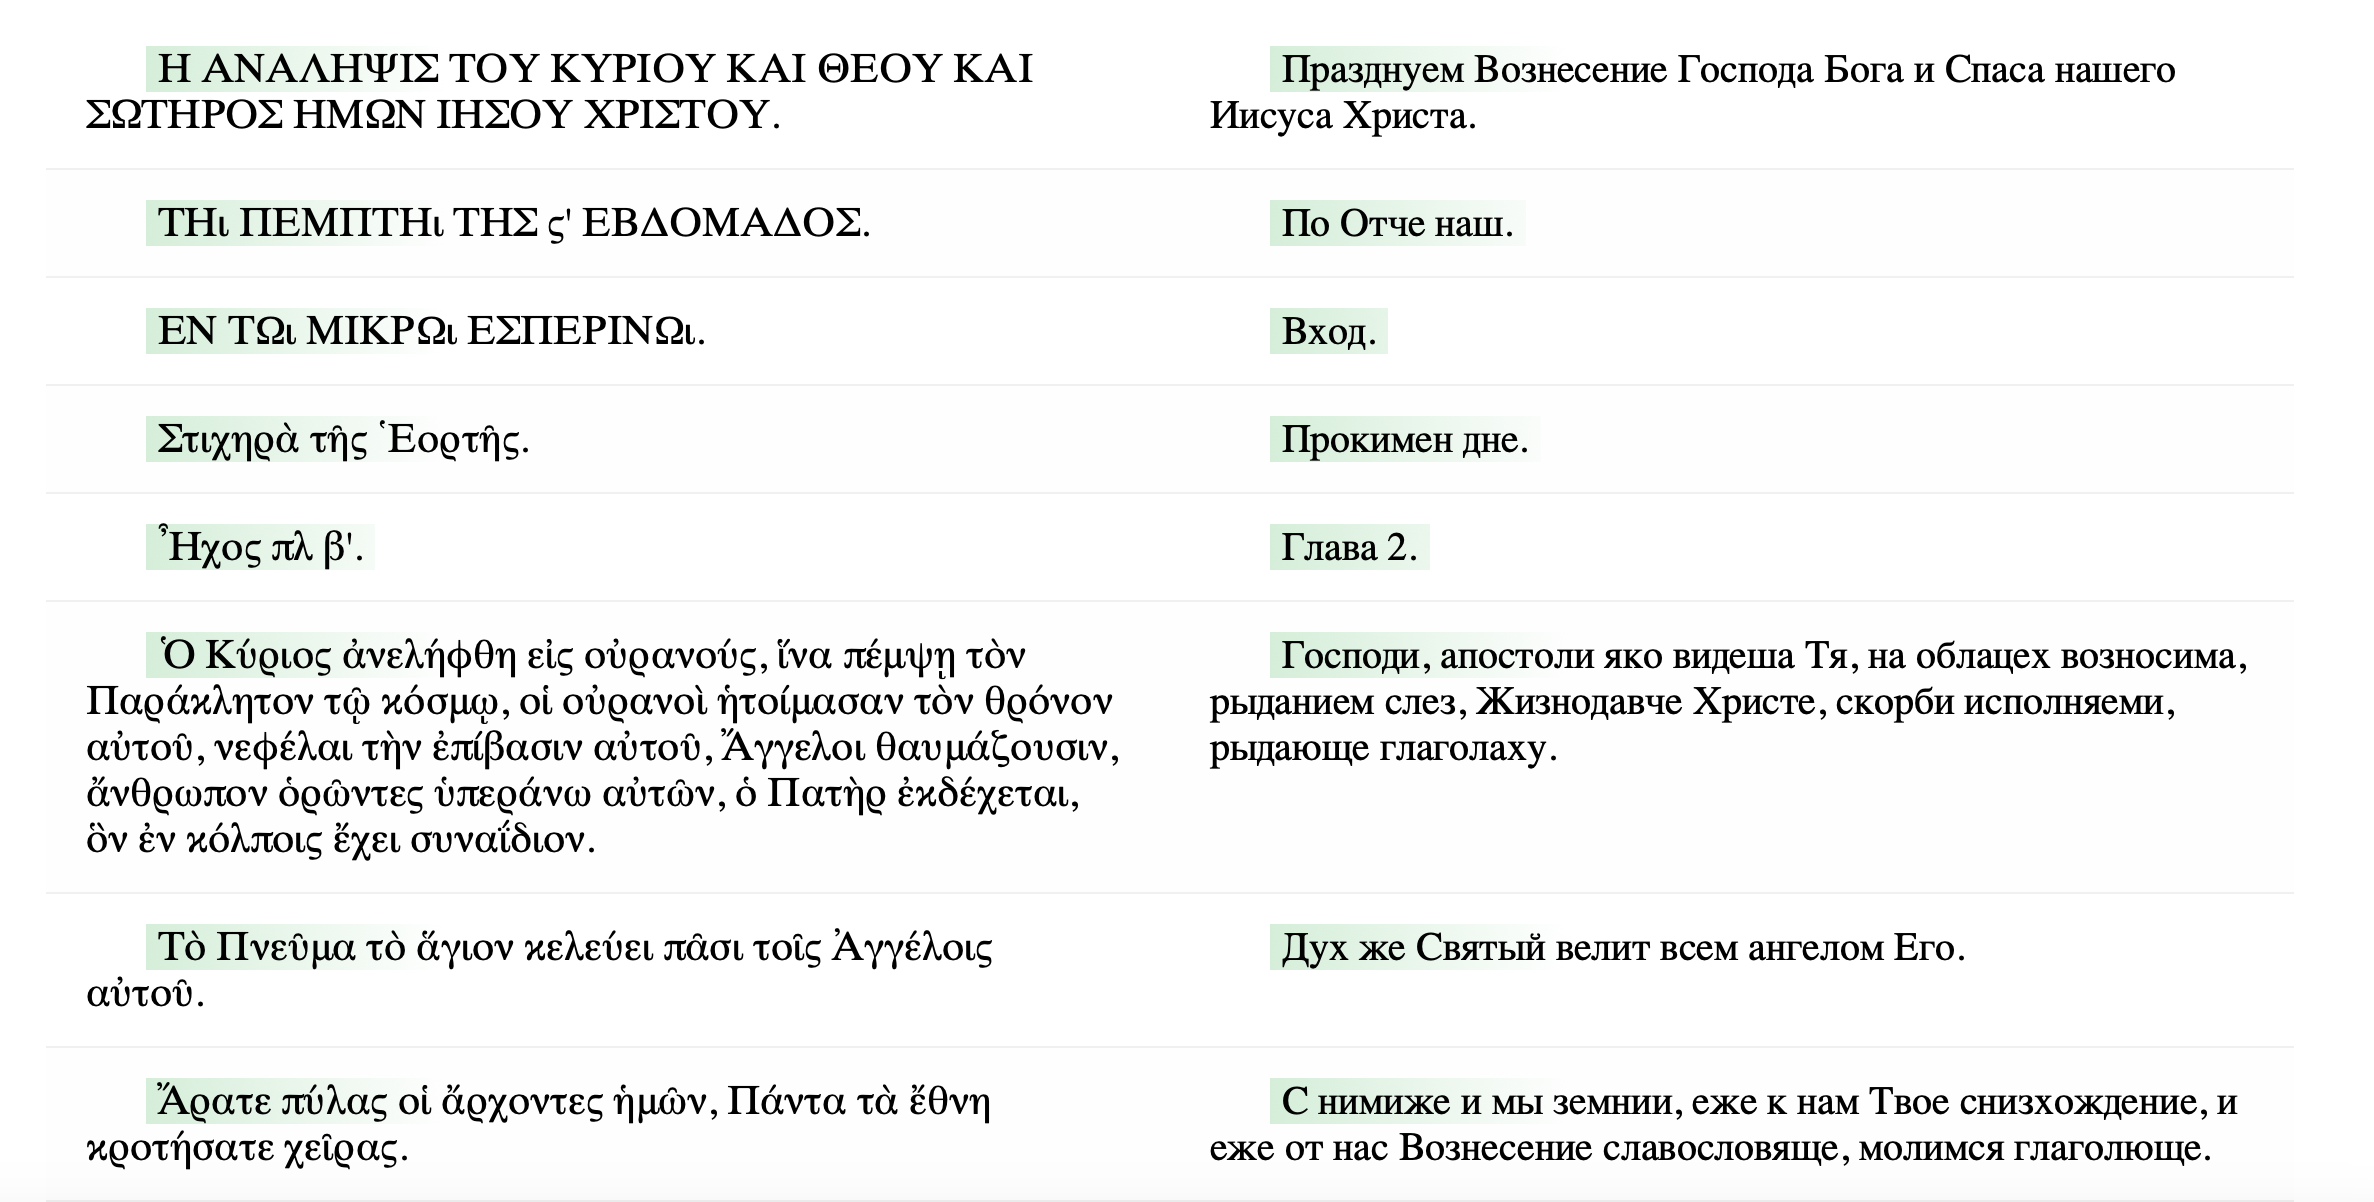
\includegraphics{images/lingtrain_faulty_result.png}

\end{tcolorbox}

\begin{tcolorbox}[enhanced jigsaw, breakable, arc=.35mm, colframe=quarto-callout-note-color-frame, leftrule=.75mm, bottomrule=.15mm, rightrule=.15mm, toprule=.15mm, opacityback=0, left=2mm, colback=white]

\textbf{Неужели элайнеры для нас совсем не годятся?}\vspace{2mm}

В процессе работы с элайнерами мы поняли, что эти инструменты не
подходят для выравнивания текстов Цветной Триоди. Будучи изначально
составленными для более очевидных задач, алгоритмы элайнеров не
справляются с темпоральной и перекрестной структурой наших текстов.

Однако, такой функционал как выдача результатов в виде html-книги с
параллельным текстом может быть актуален в контексте настоящего проекта
для оценки результатов при составлении
\protect\hyperlink{sec-about_evluation}{``золотого датасета''}.

\end{tcolorbox}

В репозитории доступен
\href{https://github.com/Drozhzhinastya/GSPC/blob/main/scripts/aligners/Lingtrain_LABse.ipynb}{код
Lingtrain} для работы с текстами Цветной Триоди.

\bookmarksetup{startatroot}

\hypertarget{ux43bux435ux43cux43cux430ux442ux438ux437ux430ux446ux438ux44f}{%
\chapter{Лемматизация}\label{ux43bux435ux43cux43cux430ux442ux438ux437ux430ux446ux438ux44f}}

\hypertarget{ux434ux43bux44f-ux447ux435ux433ux43e}{%
\section{Для чего?}\label{ux434ux43bux44f-ux447ux435ux433ux43e}}

\begin{enumerate}
\def\labelenumi{\arabic{enumi}.}
\tightlist
\item
  \emph{Лемматизация как инструмент работы с элайнерами}
\end{enumerate}

При решении задачи параллельного выравнивания текстов лемматизация может
оказаться необходимой для дальнейшей обработки текста с помощью
элайнеров или пайплайна, использующего словарь переводных эквивалентов
(в нашем случае, при работе с LF-aligner).

В других ситуациях -- например, при использовании векторных моделей
наподобие Lingtrain Aligner -- необходимость в лемматизации текстов
пропадает.

\begin{enumerate}
\def\labelenumi{\arabic{enumi}.}
\tightlist
\item
  \emph{Улучшение качества лемматизации служебных текстов может являться
  отдельной исследовательской задачей, актуальной для двух направлений
  развития проекта:}
\end{enumerate}

\begin{itemize}
\tightlist
\item
  создание словаря переводных эквивалентов
\item
  оценка и улучшение качества выравнивания текстов по предложениям
  (см.пункт `Вопрос оценки качества выравнивания')
\end{itemize}

\hypertarget{ux43bux435ux43cux43cux430ux442ux438ux437ux430ux446ux438ux44f-ux442ux435ux43aux441ux442ux43eux432-ux446ux432ux435ux442ux43dux43eux439-ux442ux440ux438ux43eux434ux438}{%
\section{Лемматизация текстов Цветной
триоди}\label{ux43bux435ux43cux43cux430ux442ux438ux437ux430ux446ux438ux44f-ux442ux435ux43aux441ux442ux43eux432-ux446ux432ux435ux442ux43dux43eux439-ux442ux440ux438ux43eux434ux438}}

\hypertarget{ux446ux435ux440ux43aux43eux432ux43dux43eux441ux43bux430ux432ux44fux43dux441ux43aux438ux439-ux442ux435ux43aux441ux442}{%
\subsection{Церковнославянский
текст}\label{ux446ux435ux440ux43aux43eux432ux43dux43eux441ux43bux430ux432ux44fux43dux441ux43aux438ux439-ux442ux435ux43aux441ux442}}

В условиях отсутствия готового модуля, позволяющего провести
лемматизацию церковнославянского текста, а также учитывая описанную
специфику Цветной Триоди, было решено попробовать лемматизировать
Триодь, экспериментируя с моделями современного русского языка (Spacy,
PyMorphy2, UDPipe), так и используя модели древних языков (UDPipe).

Результаты лемматизации Spacy и PyMorphy2 показали крайне низкое
качество, и эти инструменты были исключены из списка рассматриваемых.

Для русского языка -- современного и древнего -- в UDPipe представлено 6
моделей. В таблице ниже изложены описания данных моделей:

\begin{longtable}[]{@{}
  >{\raggedright\arraybackslash}p{(\columnwidth - 2\tabcolsep) * \real{0.5000}}
  >{\raggedright\arraybackslash}p{(\columnwidth - 2\tabcolsep) * \real{0.5000}}@{}}
\toprule\noalign{}
\begin{minipage}[b]{\linewidth}\raggedright
Модель
\end{minipage} & \begin{minipage}[b]{\linewidth}\raggedright
Тексты, корпуса, трибанки модели
\end{minipage} \\
\midrule\noalign{}
\endhead
\bottomrule\noalign{}
\endlastfoot
old\_church\_slavonic-proiel-ud-2.6-200830 & тексты старославянских
памятников, представленные в корпусе PROIEL \\
old\_russian-rnc-ud-2.6-200830 & памятники древнерусской и
церковнославянской литературы, представленные в базе Национального
корпуса русского языка \\
old\_russian-torot-ud-2.6-200830 & корпус древнерусских и
старославянских текстов Torot \\
russian-syntagrus-ud-2.6-200830 & художественные тексты и новостные
издания современного русского языка аннотированного корпуса SynTagRus \\
russian-gsd-ud-2.6-200830 & конвертированный корпус Google Stanford
Dependencies \\
russian-taiga-ud-2.6-200830 & художественные, новостные, научные
датасеты, субтитры и поэзия современного русского языка, представленные
в корпусе Taiga \\
\end{longtable}

Для оценки качества моделей, каждая из них была использована при
лемматизации тестового фрагмента Триоди -- текста службы Вознесения
{[}ССЫЛКА{]}.

Наименее удовлетворительные результаты были получены при работе с
церковнославянской моделью
\emph{old\_church\_slavonic-proiel-ud-2.6-200830}. Модели, основанные на
корпусах Torot и RNC проявили себя лучше. Однако, Torot оказалась
чувствительной к знакам препинания -- при работе с этой моделью текст
нуждается в предварительном удалении пунктуации.

Ошибки лемматизации были в основном общие -- например, парсеру не
удалось правильно построить инфинитивы предиката \emph{празднуем} и
\emph{глаголет}. С \emph{глаголет} не справились и современные модели
(SynTagRus, GSD, Taiga). В целом результаты последних были довольно
ровными, хотя с некоторыми словоформами Taiga справлялась лучше, чем
SynTagRus и GSD. Например, ей удалось распарсить словоформу
\emph{вечерни (вечерня)}, с которой из других моделей справилась только
Torot.

Помимо проблемы правильного построения начальной формы, возникли ошибки,
связанные с омонимией. Так, модели GSD и Taiga, к примеру, не всегда
могли принять правильное решение о начальной форме аккузатива и генитива
существительного \emph{Господь} (\emph{Господа}), совпадающей с
номинативом множественного числа \emph{господин.} Лучшие результаты
показала модель \emph{SynTagRus}.

---\textgreater{} При распространении лемматизации на полный текст
Триоди необходимо выявить модель с наилучшим качеством. По результатам
экспериментов мы решили отказаться от PROIEL, а из современных моделей
выбирать между Taiga и SynTagRus, хотя их качество при лемматизации
службы одного дня оказалось не совсем идеальным.

\emph{\href{https://github.com/Drozhzhinastya/GSPC/tree/main/scripts/lemmatization}{Код}
и
\href{https://github.com/Drozhzhinastya/GSPC/tree/main/lemmatization/csl}{результаты}
лемматизации}

\hypertarget{ux433ux440ux435ux447ux435ux441ux43aux438ux439-ux442ux435ux43aux441ux442}{%
\section{Греческий
текст}\label{ux433ux440ux435ux447ux435ux441ux43aux438ux439-ux442ux435ux43aux441ux442}}

Для лемматизации древнегреческого текста используется модуль Backoff
Lemmatizer библиотеки CLTK. Выбор лемматизатора основан на выводах,
представленных в статье McGillivray-Vatri, авторы которой анализируют
точность четырех программных решений для лемматизации текста: Diorisis,
LAGT, GLEM, и CLTK. По результатам двух серий экспериментов CLTK показал
сравнительно высокую точность подбора корректной леммы, что и послужило
определяющим фактором при выборе данного модуля для работы в рамках
проекта.

Другим очевидным преимуществом \emph{backoff} модуля является
использование цепочки лемматизаторов: в случае неудачного результата при
обработке токена программа обращается ко внешним лемматизаторам, пока не
будет найдена лемма или не будут исчерпаны все указанные варианты.
Данный подход существенно повышает точность обработки текста, однако
имеет и определенные недостатки. Поскольку backoff-цикл прерывается при
первой найденной лемме, результаты лемматизации будут сильно отличаться
в зависимости от того порядка, в котором указаны внешние лемматизаторы в
backoff-цепочке.

В качестве экспериментальных корпусов в проекте McGillivray-Vatri
использовались классические тексты, что актуализирует проблему
идентификации языка текста Цветной Триоди.

Библиотека CLTK, как и прочие аналогичные инструменты, направлена на
обработку классических текстов, а модели Backoff Lemmatizer для
древнегреческого языка обучены на материалах проекта Perseus. Греческий
текст Цветной Триоди, обрабатываемый в рамках проекта, довольно сложно
поддается лингвистической классификации -- необходим более глубокий
анализ и консультация специалистов, чтобы выйти за рамки
сформулированного внутри проекта условного обозначения \emph{греческий
язык богослужебных текстов}. Как и в случае с условно церковнославянским
текстом, греческая Триодь находится на шкале между койне и греческим
Нового Завета, сочетая элементы обеих форм греческого языка.

Ниже представлены результаты лемматизации греческого фрагмента службы
Вознесения при помощи лемматизаторов CLTK и UDPipe, а также фрагмент
исходного текста для сравнения:

\begin{itemize}
\tightlist
\item
  Исходный текст:
\end{itemize}

\emph{Ὁ Κύριος ἀνελήφθη εἰς οὐρανούς, ἵνα πέμψῃ τὸν Παράκλητον τῷ κόσμῳ,
οἱ οὐρανοὶ ἡτοίμασαν τὸν θρόνον αὐτοῦ, νεφέλαι τὴν ἐπίβασιν αὐτοῦ,
Ἄγγελοι θαυμάζουσιν, ἄνθρωπον ὁρῶντες ὑπεράνω αὐτῶν, ὁ Πατὴρ ἐκδέχεται,
ὃν ἐν κόλποις ἔχει συναΐδιον. Τὸ Πνεῦμα τὸ ἅγιον κελεύει πᾶσι τοῖς
Ἀγγέλοις αὐτοῦ· Ἄρατε πύλας οἱ ἄρχοντες ἡμῶν, Πάντα τὰ ἔθνη κροτήσατε
χεῖρας. ὅτι ἀνέβη Χριστός, ὅπου ἦν τὸ πρότερον.}

\begin{itemize}
\tightlist
\item
  CLTK:
\end{itemize}

\emph{ὁ κύριος ἀναλαμβάνω εἰς οὐρανός ἵνα πέμπω ὁ παράκλητος ὁ κόσμῳ, ὁ
οὐρανός ἑτοιμάζω ὁ θρόνος αὐτός νεφέλη ὁ ἐπίβασις αὐτός ἄγγελος θαυμάζω
ἄνθρωπος ὁράω ὑπεράνω αὐτός ὁ πατήρ ἐκδέχομαι ὅς ἐν κόλπος ἔχω συναΐδιον
ὁ πνεῦμα ὁ ἅγιος κελεύω πᾶς ὁ ἄγγελος αὐτός ἀείρω πύλη ὁ ἄρχων ἡμεῖς πᾶς
ὁ ἔθνος κροτέω χείρ ὅτι ἀναβαίνω χριστός ὅπου εἰμί ὁ πρότερος}

\begin{itemize}
\tightlist
\item
  UDPipe - Perseus
\end{itemize}

\emph{ὁ Κύριος ἀαλαμβάνω εἰς οὐρανός, ἵνα πέμπω ὁ Παράκλητος ὁ κόσμος ,
ὁ οὐρανός ἑτοιμάζω ὁ θρόνος αὐτός , νεφέλα ὁ ἐπίβασις αὐτός , Ἄγγελοι
θαυμάζω , ἄνθρωπος ὁράω ὑπεράνω αὐτός , ὁ Πατὴρ ἐκδέχομαι , ὅς ἐν κόλπος
ἔχω συναΐδιος ὁ Πνεῦμα ὁ ἅγιος κελεύω πᾶς ὁ Ἀγγέλοί αὐτός · Ἄρατε πύλη ὁ
ἄρχων ἐγώ , πᾶς ὁ ἔθνος κροτάω χείρ ὅτι ἀνέβη Χριστός , ὅπου εἰμί ὁ
πρότερος}

Как видно из примеров, оба лемматизатора показывают довольно высокую
точность. CLTK не справился со словом \emph{ὁ κόσμος} (здесь в значении
«мир»), оставив его в форме дательного падежа. Возможной причиной ошибки
может являться \emph{iota subscriptum} (подстрочная йота),
встречающаяся, среди прочего, в формах существительных дательного
падежа. Потенциальным решением подобной проблемы может быть замена таких
букв на формы \emph{iota adscriptum} на этапе предварительной обработки
текста: ῳ --\textgreater{} ωι.

Фрагмент, обработанный при помощи UDPipe, содержит больше неточностей:
диалектная форма \emph{νεφέλα} вместо ожидаемого \emph{νεφέλη}
(«облако»), пропущенная буква «ню» в глаголе

\emph{ἀαλαμβάνω} (здесь «возношусь»), а также необработанные формы
\emph{ἄρατε} (\emph{αἴρω}, \emph{ἀείρω}, «поднимаю, беру») и
\emph{ἀνέβη} (\emph{ἀναβαίνω}, «восхожу»). При этом, UDPipe распознает
именованные сущности, что может оказаться актуальным, если будет решено
добавить подобный функционал в пайплайн.

\emph{\href{https://github.com/Drozhzhinastya/GSPC/tree/main/scripts/lemmatization}{Код}
и
\href{https://github.com/Drozhzhinastya/GSPC/tree/main/lemmatization/greek}{результаты}
лемматизации}

\bookmarksetup{startatroot}

\hypertarget{text-similarity}{%
\chapter{Text-similarity}\label{text-similarity}}

Задача оценки семантического сходства (text-similarity) заключается в
определении степени схожести двух предложений с точки зрения
транслируемого смысла.

Семантический поиск направлен на повышение точности сопоставления
текстовых единиц путем понимания содержания поискового запроса. В
отличие от использования только лексических совпадений, семантический
поиск также может находить синонимы и другие единицы, имеющие схожий
контекст употребления, поскольку этот алгоритм основывается на
эмбеддингах -- векторных представлениях текстовых единиц. Термин
``embedding'', взятый из английской литературы, используется для
описания процесса, когда модель оцифровывает смысл слов и записывает его
в виде упорядоченного набора числовых значений -- вектора.

Наиболее эффективным способом построения моделей естественного языка
является обучение нейронных сетей на основе архитектуры «трансформер». В
качестве примера можно привести
\href{https://arxiv.org/abs/1810.04805}{BERT} -- модель. которая
используется для определения сходства слов и предложений.

Более качественные результаты можно получить, оптимизируя BERT под
конкретные задачи. К примеру, модель
\href{https://arxiv.org/pdf/1908.10084.pdf}{SBERT} обучена
непосредственно для работы с задачами по определению схожести
предложений на основе косинусной меры.

Как отмечают разработчики
\href{https://habr.com/ru/companies/sberdevices/articles/527576/}{модели},
её ``архитектура представляет собой
\href{https://en.wikipedia.org/wiki/Siamese_neural_network}{сиамскую
нейронную сеть} с тремя входами для триплета~ «anchor --- positive ---
negative».~ К каждому из входов применяется модуль BERT, который и будет
выполнять роль NLU в этом эксперименте. Модуль содержит в себе
\href{https://paperswithcode.com/method/wordpiece}{wordpiece-токенизатор}
для преобразования входных строк в BERT-совместимый формат (input\_ids,
input\_mask, token\_type\_ids), а также саму обучаемую модель BERT для
векторизации текста.''

В результате дообучения модели SBERT для задачи поиска переводных
эквивалентов было получено множество вариантов
\href{https://huggingface.co/models?pipeline_tag=sentence-similarity\&sort=downloads\&search=multi}{мультиязычных
моделей}.

В настоящий момент мы считаем, что подобные мультиязыковые модели могут
значительно приблизить проект к решению изначальной задачи, потенциально
обеспечивая более высокое качество поиска наиболее схожих единиц
греческого и церковнославянского текста.

В репозитории представлен
\href{https://github.com/Drozhzhinastya/GSPC/blob/main/scripts/text-similarity/GSPC_sbert.ipynb}{код}
для работы с нашим текстом, а также результаты работы с моделью
sentence-transformers/all-MiniLM-L6-v2, которая на наш взгляд
демонстрирует более высокое качество сведения текстов Триоди.

Эксперименты проводились как на уровне отдельных предложений, так и на
уровне гимнов (минимальных единиц разметки текста, представленной в
нашей csv - см.выше). Каждое уникальное предложение/гимн греческого
текста сопоставлялось с каждым предложением церковнославянского текста.
Результаты экспериментов представлены в
\href{https://github.com/Drozhzhinastya/GSPC/tree/main/csv/sbert}{csv
таблице}, где собраны топ-5 церковнославянских предложений, выделенных
моделью как наиболее близкие соответствующему греческому элементу.

В дальнейшей перспективе предстоит разработать решение для оценки
качества сведения текстов и улучшения результатов выравнивания с опорой
на него.

\bookmarksetup{startatroot}

\hypertarget{sec-about_evluation}{%
\chapter{Вопрос об оценке качества сведения
текстов}\label{sec-about_evluation}}

В этой связи на настоящий момент мы выявили 3 основных метода для оценки
качества результатов сведения потенциально эквивалентных единиц, каждый
из которых, тем не менее требует оптимизации:

\begin{itemize}
\tightlist
\item
  Качественный отсмотр результатов работы моделей и элайнеров
  специалистами (ресурсозатратно)
\item
  Создание золотого датасета / готового датасета выровненных текстов,
  который может быть использован для оценки качества выравнивания (в
  отличие от Цветной Триоди, результатов выравнивания которой в готовом
  виде нет). В качестве источника создания такого датасета могут быть
  использованы выровненные тексты
  \href{https://dhonorare.ru/texts/trebnik/molitvy-v-pervyy-den-posle-rozhdeniya-mladentsa}{DHonorare}
\item
  Создание золотого датасета + дообучение наиболее оптимальных моделей
  BERT на нём
\end{itemize}

\bookmarksetup{startatroot}

\hypertarget{ux43dux430ux43fux440ux430ux432ux43bux435ux43dux438ux44f-ux434ux430ux43bux44cux43dux435ux439ux448ux435ux433ux43e-ux438ux441ux441ux43bux435ux434ux43eux432ux430ux43dux438ux44f}{%
\chapter{Направления дальнейшего
исследования}\label{ux43dux430ux43fux440ux430ux432ux43bux435ux43dux438ux44f-ux434ux430ux43bux44cux43dux435ux439ux448ux435ux433ux43e-ux438ux441ux441ux43bux435ux434ux43eux432ux430ux43dux438ux44f}}

Не смотря на то, что изначальные исследовательские цели не
финализированы, работа над проектом проявила множество
особенностей/проблемных зон/вопросов, требующих дальнейшего уточнения.

Проект продолжается; мы продолжаем исследовать обозначенные методы и
инструменты, а также искать новые решения, которые могут приблизить нас
к искомому результату.

\begin{itemize}
\tightlist
\item
  оптимизация алгоритма проверки качества сведения текстов
\item
  выравнивание текстов Цветной триоди с оценкой качества
\item
  публикация параллельного корпуса на самостоятельной платформе или
  интеграция в \href{https://liturcorpora.ru/}{Liturcorpora}
\end{itemize}


\backmatter

\end{document}
